\documentclass{article}

\usepackage[backend=bibtex,style=numeric, citestyle=ieee]{biblatex}
\addbibresource{bibliography.bib}

\usepackage{amsmath}
\usepackage{pgfgantt}
\usepackage[noend]{algpseudocode}
\usepackage[]{algorithm2e}
\usepackage{graphicx}
\usepackage{float}
\usepackage{hyperref}
\usepackage{titlesec}
\usepackage[
top    = 2.50cm,
bottom = 2.50cm,
left   = 2.75cm,
right  = 2.75cm]{geometry}
\usepackage{fancyhdr}
\pagestyle{fancy}
\lhead{COMP3003 - Interim Report }
\rhead{Jonathan Foot - psyjpf}

\newcommand{\CS}{C\nolinebreak\hspace{-.05em}\raisebox{.6ex}{\tiny\bf \#}}




\begin{document}
\pagenumbering{roman}
\begin{titlepage}
	\begin{center}
		\vspace*{1cm}
		\Huge
		\textbf{A Data-Driven Approach To Bus Timetable Optimisation Recommendations.a}
		
		\LARGE
		\vspace{0.5cm}
		\textbf{Interim Report}
		
		\vspace{1.5cm}
				
		\textbf{Jonathan Foot}
		
		School of Computer Science
		
		psyjpf@nottingham.ac.uk
		
		
		\vspace{2.5cm}
		
		An interim report for the degree of\\
		MSci Computer Science
		
		
		\vfill
		
		
\includegraphics[width=200px]{images/nottingham-logo.png}
	\end{center}
\end{titlepage}

\tableofcontents


\newpage

\setcounter{page}{1}
\pagenumbering{arabic}
% Do all this to reduce the page count ;) 
\setlength{\parindent}{2em}
\setlength{\parskip}{1em}
\setlength{\belowcaptionskip}{-10pt}
\titlespacing\section{0pt}{12pt plus 4pt minus 2pt}{0pt plus 2pt minus 2pt}
\titlespacing\subsection{0pt}{12pt plus 4pt minus 2pt}{0pt plus 2pt minus 2pt}
\titlespacing\subsubsection{0pt}{12pt plus 4pt minus 2pt}{0pt plus 2pt minus 2pt}


\section{Introduction and Motivation}


Bus transit systems remains the UK's leading public transportation method, with the average UK resident making 48 trips annually \cite{RN9}. Bus networks allow for a relatively low initial infrastructural investment, while offering great adaptability and environmental benefits; particularly with the popularity of hydrogen, electric and bio-gas buses increasing. Although, private transportation methods still remain the UK's preferred method of transport, with the average person taking 602 trips by car \cite{RN9}, over 12 times that of the number of bus trips. 

\par
One of the leading deterrents for greater adoption of bus transportation is ``a belief that buses cannot be relied on to stick to their timetables''\cite{RN10}. Transport operators are responsible for the network route design, setting the frequencies, timetables and assigning vehicles and drivers to trips. When creating the timetable operators must consider both external factors, such as traffic, roadworks, severe weather, sporting events and internal factors, such as delays from previous trips affecting the subsequent trips and delays on passenger boarding and alighting \cite{RN11}.

\par
The UK Senior Traffic Commissioner’s guidelines are for 95\% of buses to be “on-time”, which is defined as arriving between 1 minute early to 5 minutes late at a timing point\cite{RN14}. If bus operators repeatedly fail to adhere to this guideline, they can be fined up to £550 per vehicle \cite{RN14}. One way to ensure compliance is to add a significant amount of excess wait times at stops to recoup for any delays. But this will increase journey times and unneeded waiting can be considered “dead time” where the bus operator is not making any money. Creating a reliable timetable is therefore important to both the operators and customers alike.


\par
98\% of buses in Great Britain are equipped with automatic vehicle location (AVL) devices\cite{RN12}, which is used to monitor the punctuality of buses to a high degree of accuracy. With some operators even storing the exact longitudinal and latitudinal position of every bus, up-to every 30 seconds. There is more data about buses than ever-before and with the United Kingdom Government legislating the Bus Service Act 2017\cite{RN13}, bus open data is becoming increasingly more accessible. It is my intentions that this open-data can be used to drive an optimisation algorithm to make new timetable recommendations, improve average on-time performance and instil greater customer confidence in bus timetables and using buses as a form of transport.



\section{Related Work}
There is already a plethora of work on public transit systems, which can be categorised into five key parts \cite{RN18} \cite{RN20}, (1) transportation route network design (TRND), (2) timetable setting (3) crew scheduling (4) vehicle scheduling (5) real-time control during service. Timetable Setting has further been popularised into following optimisation objectives\cite{RN7}: (1) minimising average wait time (2) minimising transfer times between routes (3) minimising total travel time (4) Balancing of operators cost with users benefits. 

 \par
Transportation route network design involves defining each line's route, length, stop density and key defining characteristics, such as proposed general frequency. Setting of the timetable, defines when the each bus will leave the first bus stop and takes into consideration the uncertainty of passengers' demands and travel times, due to external and internal factors\cite{RN11}. Considerations should also be made for connections between other lines, train times, school times, \textsl{et al}. This can be even further complicated by having multiple bus depots, (often referred to as the Multiple Depot Vehicle Scheduling Problem), considerations for staff changeover locations and breaks, minimisations of dead-heading travels, utilisation of bus-lanes and bus-gates, unplanned vehicle maintenance, roadworks and changes in fuel prices. 

\par 
Setting and evaluating a bus timetable can therefore be described as an NP-Hard problem \cite{RN15}. Due to the complexity of the task many people choose to target only one or two aspects of the problem at a time. As it is impractical to believe a single algorithm could generate a perfect new timetable, considering all possible factors.

\par
Data-driven approaches have only started being researched relatively recently, which I suspect is because the quality and accessibility of the data has only become viable in the last decade, with 2010 being the first year where over half of buses in the UK had AVL\cite{RN12}. As such there is a limited number of papers on my exact proposal.

\par
 One such paper however is proposed by Jinjun Tang \textsl{et al} who used a multi-objective genetic algorithm \cite{RN18}, to minimise the passenger waiting time, whilst also reducing the total number of departures; to ensure the number of vehicles need to operate the service during peak times was not significantly greater than non-peak times, for greater utilisations of vehicle resources. Like me they proposed a data-driven approach, however they used Smart Card and GPS Data to understand passenger demand and travel times. Furthermore, they added vehicle capacity as one of their constraints.

\par
Fangzhou Sun \textsl{et al} proposed a single-objective greedy and genetic algorithm (GA)\cite{RN8}, to increase a services' on-time percentage by minimising slack times. With the constraint that the last time point of a trip must always be the first time point of the next i.e. every trip must follow on from the last. Like me they are also using a data-driven approach using historical time-point feed data and schedule data. However, unlike me they assume that the arrival and departure time will always be the same, so no consideration for boarding time is made. They found that a GA was more effective than a Greedy algorithm.  

\par
Sanchita Basak \textsl{et al} similarly proposed a single-objective optimisation task, with a greedy, genetic and particle swarm optimisation algorithm (PSO), with the ``objective of maximizing probability of bus arrivals at time points with delays within desired on-time ranges''\cite{RN7}, using  historical time-point data and real-time information. Unlike the other to two data-driven approaches they focused more on the seasonal difference and monthly grouping of patterns throughout the year. They also discovered that a PSO executed faster than a GA, while producing similar results.


\par 
Friedman proposed one of the earliest time table scheduling solutions in 1975\cite{RN22} , representing the problem as a mathematical programming model, with the aim to minimise average passenger waiting time; considering constraints on allocations of drivers and vehicles. Although he relied upon known deterministic conditions such passenger numbers and traffic intensity, an unrealistic assumption to make.

\par 
Daniel Sun \textsl{et al} used a heuristic algorithm to look at how different capacity buses could be used to deal with demand fluctuations  \cite{RN32}. Ceder and Lucas, looked at creating a timetable to minimise bus overcrowding \cite{RN33}. Yinghui Wu \textsl{et al} proposed an integer-programming model and a genetic-algorithm with a local search to optimise the slack times in a timetable and reduce randomness \cite{RN26}, by focusing on three types of passengers, those transferring, boarding and currently travelling. Some have attempted optimising the TRND and timetables simultaneously with a GA to minimise travel and transfer times \cite{RN23}\cite{RN31}. 
 
\subsection{Under-researched areas}
 
While there is already a lot of research and proposed methods into the different areas of timetable optimisation. One area which has not been focused upon as much is considerations for routes which share the same common path for a portion of their routes before separating off. This is particularly common for urban areas, where local councils may have invested into bus lanes, bus gates or less popular sump busters. Due to the road space invested into them and their ability to reduce travel times \cite{RN34}, they lend themselves to encourage multiple services to share the same route-segment. These shared route-segments across several services have been coined ``bus corridors'' by some.

\par
When multiple services share a common route-segment, passengers may not be concerned about which of the services they board on, if they do not wish to travel past their shared segment. Instead they will choose to travel on which ever service arrives first at their stop. It is this phenomenon I wish to explore further.


\section{Description of the work}

I intend to create a program which given a set of historical timetable and vehicle times can return back an improved optimised timetable, based upon four optimisation criteria. The end-user of the program is bus-operators, to use internally at time-table reviews, with the desired outcome that it enables them to make more informed decisions.


\par
The program will let the bus-operator review their services' current performance metrics such as percentage on-time performance (also know as timepoint schedule adherence) and cohesion with other services' which share a common route-segment. The program will let them select a service and choose to optimise it.
\par
Once selected the program will find the points in the year where the timetable for a service changed, the bus-operator can then select one or several time-periods to generate a new optimised timetable. It is assumed that the performance of the timetable last-year will remain generally consistent the following year and this will account for seasonal differences. 
\par 
Once the operator has selected a bus service to optimise the program will make suggestions for other services which share a same common route-segment between them. The user can then select none or several of the suggested services, to also optimise their timetables and enabled for better cohesion between them. Such that, the headway time between services at a stop is more uniform. 
\par 
The program will then ask the user if they have any key bus stop and time pairings of interest, for example a bus stop outside a school at 8:30. These can be considered “targets” which the optimise algorithm will try to schedule a bus service to arrive at as close to the designated time as possible. The optimisation algorithm will also try to minimise any unneeded ideal/slack time at timing points. 

\par
Finally, it will give a higher ``score'' to a solution with the fewest number of changes, this is to prevent an overzealous solution and because it is difficult to be able to confidently predict how it is likely to perform. The user is then asked to order the optimisation targets based on importance and can change key parametrised values. The program will then execute and return back a set of new optimised timetables, along with a predicted set of performance metrics to allow you to compare against the previous timetable.

\subsection{Optimisation Criteria}
The four optimisation targets can therefore be summarised as:
\begin{itemize}
	\item Minimise the unneeded slack time at timing points, while balancing the percentage of buses predicted to be ``on-time''.
	\item Minimise the number of total changes and the severity of the changes, aiming to keep the timetable as close to the original as possible. Too many changes at once make it very difficult to be able to reliably predict how it is likely to function. 
	\item Maximise the uniform distribution of different services arriving at the same stop, by spreading out headway times. To do this I must identify routes which share a common route-segments.
	\item Maximise as many services as possible, to arrive at a particular set of stops and time points of interest as close as possible, this should be user-settable. For example, target for a bus arriving at a stop outside a school just before start time.
\end{itemize}
 
 The importance/ weighting (pareto dominance) of the four optimisation targets will be parameterised, such that the user can optimise a timetable based on what is most important to them, or to experiment with several timetable ideas. This is because the program will produce a pareto solution, to have the highest percentage of on-time buses you would need to increase the slack time. Similarly by increasing the number of service which arrive as close to a specific time as possible you minimise the uniform distribution of the services; as such a careful balance must be found.


\subsection{Aims and Objectives}
\begin{enumerate}
	\item Interface with the Reading Buses Open Data API, request and download data required from the API.
	\item Search through the data for weekly patterns and group them, to create multiple-timetables for the year; one for each group.
	\item Generate the performance metrics, such as average on-time performance of the old timetable for the previous year.
	\begin{enumerate}
		\item Use these metrics, to compare and contrast against the new timetable later. 
	\end{enumerate}
	\item Take in the historic vehicle data and generate a new optimised timetable, to minute accuracy.
	\begin{enumerate}
		\item Explore multiple different methods for timetable optimisation.
		\item The new timetable will try to minimise unneeded idle/dead time at timing points.	
		\item The new timetable will not consider constraints on number of vehicles, or drivers available. 
		\item The new timetable will not consider how these changes might affect connections between other routes timetables.
		\item The new timetable must bear some resemblance to the original headway times and will be restricted to prevent an overzealous solution.  
		\item The new timetable cannot alter the bus services route design.
		\item The optimisation strategy must consider the times of other services, which share a common pathway.
		\item The optimisation strategy must allow the user to input key locations and timings of particular importance. For example school starting time at a stop outside a school.
		\item The optimisation algorithm should allow for the parameters and constrains to be edited by the end-user.
	\end{enumerate}
	\item Produce a simulation/scoring system which can take in the proposed timetable and output estimated performance levels, to allow for comparison with original timetable.
	\item Create a user friendly GUI, which can graphically highlight the differences between the two timetables, to easily distinguish where the improvements have been made.  
\end{enumerate}


\section{Design and Methodology}

In the following section I will outline the overall design of the program, both from the end-users prospective, with the GUI and parts of the internal system, such as data-schemas, technologies chosen and algorithm designs.


\subsection{Chosen Technologies}
For this project I have chosen to use \CS, .NET 5, with Visual Studio 2019 Enterprise. This is because \CS, particularly with the latest .NET version offers the speed and versatility required to be able to quickly process large volumes of data. Whilst also being syntactically an easy language to develop in, particularly with the use of LINQ. Which allows for me to be able to declaratively query complex data structures with ease. Visual Studio also offers industry leading debugging tools to speed up development further. Moreover, it is my strongest programming language and as such I can be confident on my proposed implementation strategies and estimated time-lines.

\subsection{Graphical User Interface}

Figure ~\ref{fig:gui1} and ~\ref{fig:gui2} shows my preliminary GUI designs, I have focused upon creating a functional, easy to use and intuitive program layout. However, they are subject to change based upon real-world usage tests and prototyping.  

\begin{figure}[H]
	\centering
	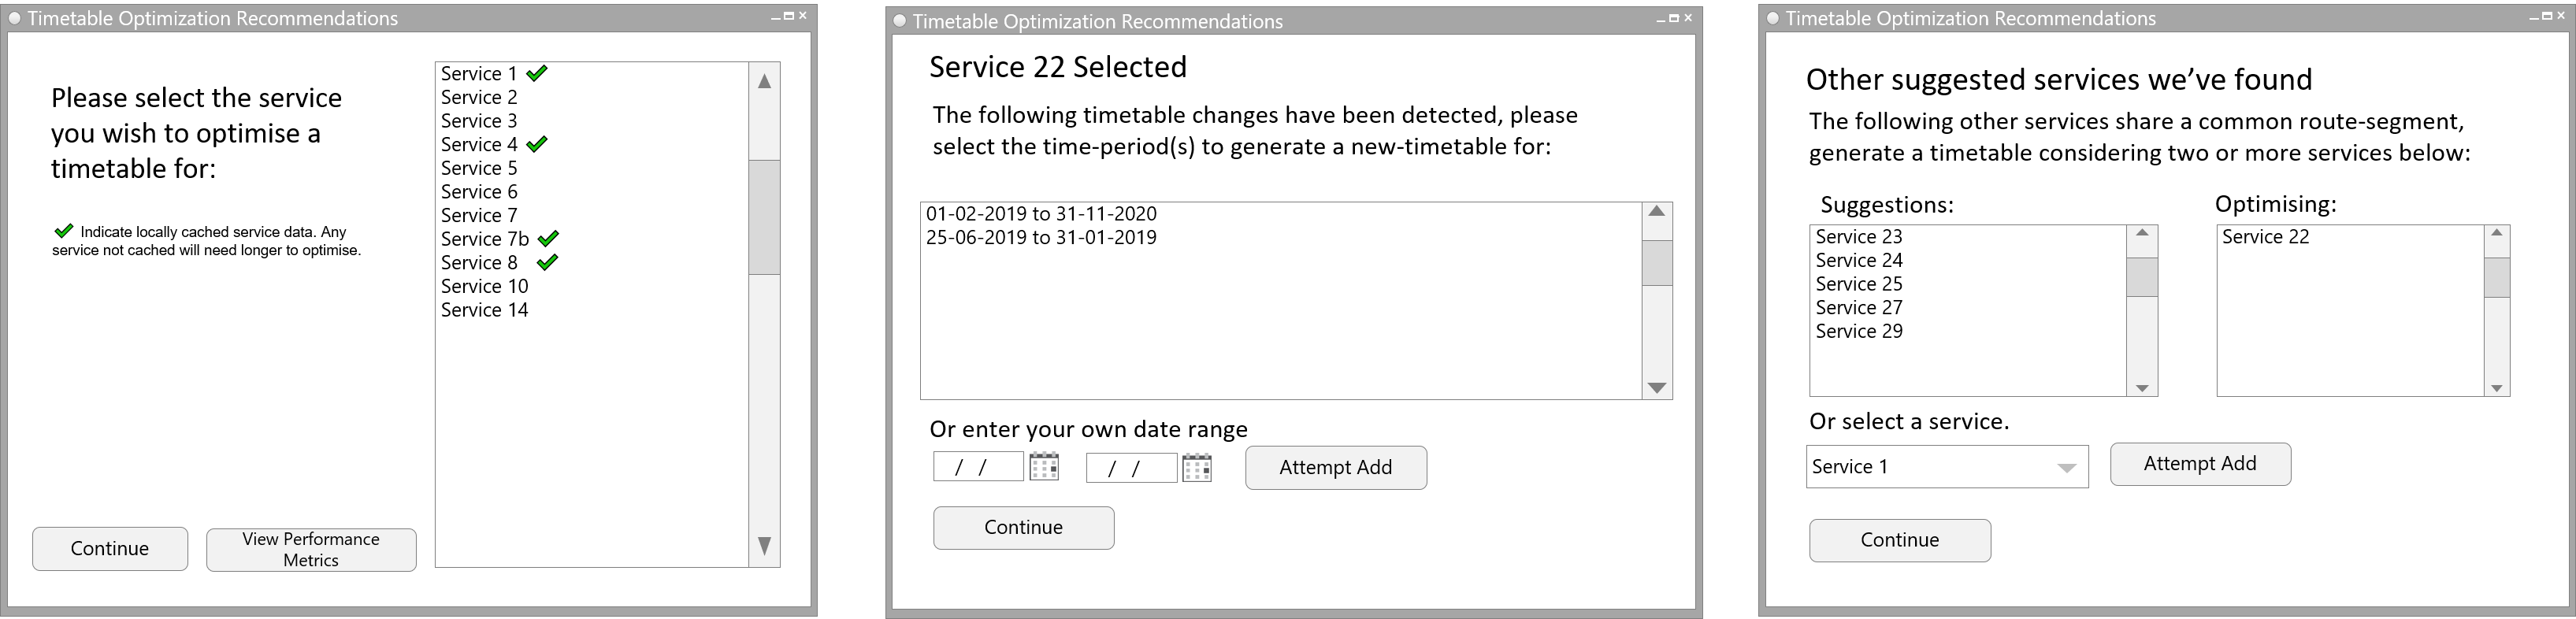
\includegraphics[height=105px]{images/GUI_1.png}
	\caption{GUI Design for Screens 1 to 3.}
	\label{fig:gui1}
\end{figure}

The start screen, lets the user select the service they want to generate a new timetable for (or to view its current performance metrics), the second screen lets you select a time-period for when the new timetable would be in effect for. The third screen lets the user see routes that share common-route segments with their selected route and can then optimise several timetables concurrently to harmonise their coordination. 


\begin{figure}[H]
	\centering
	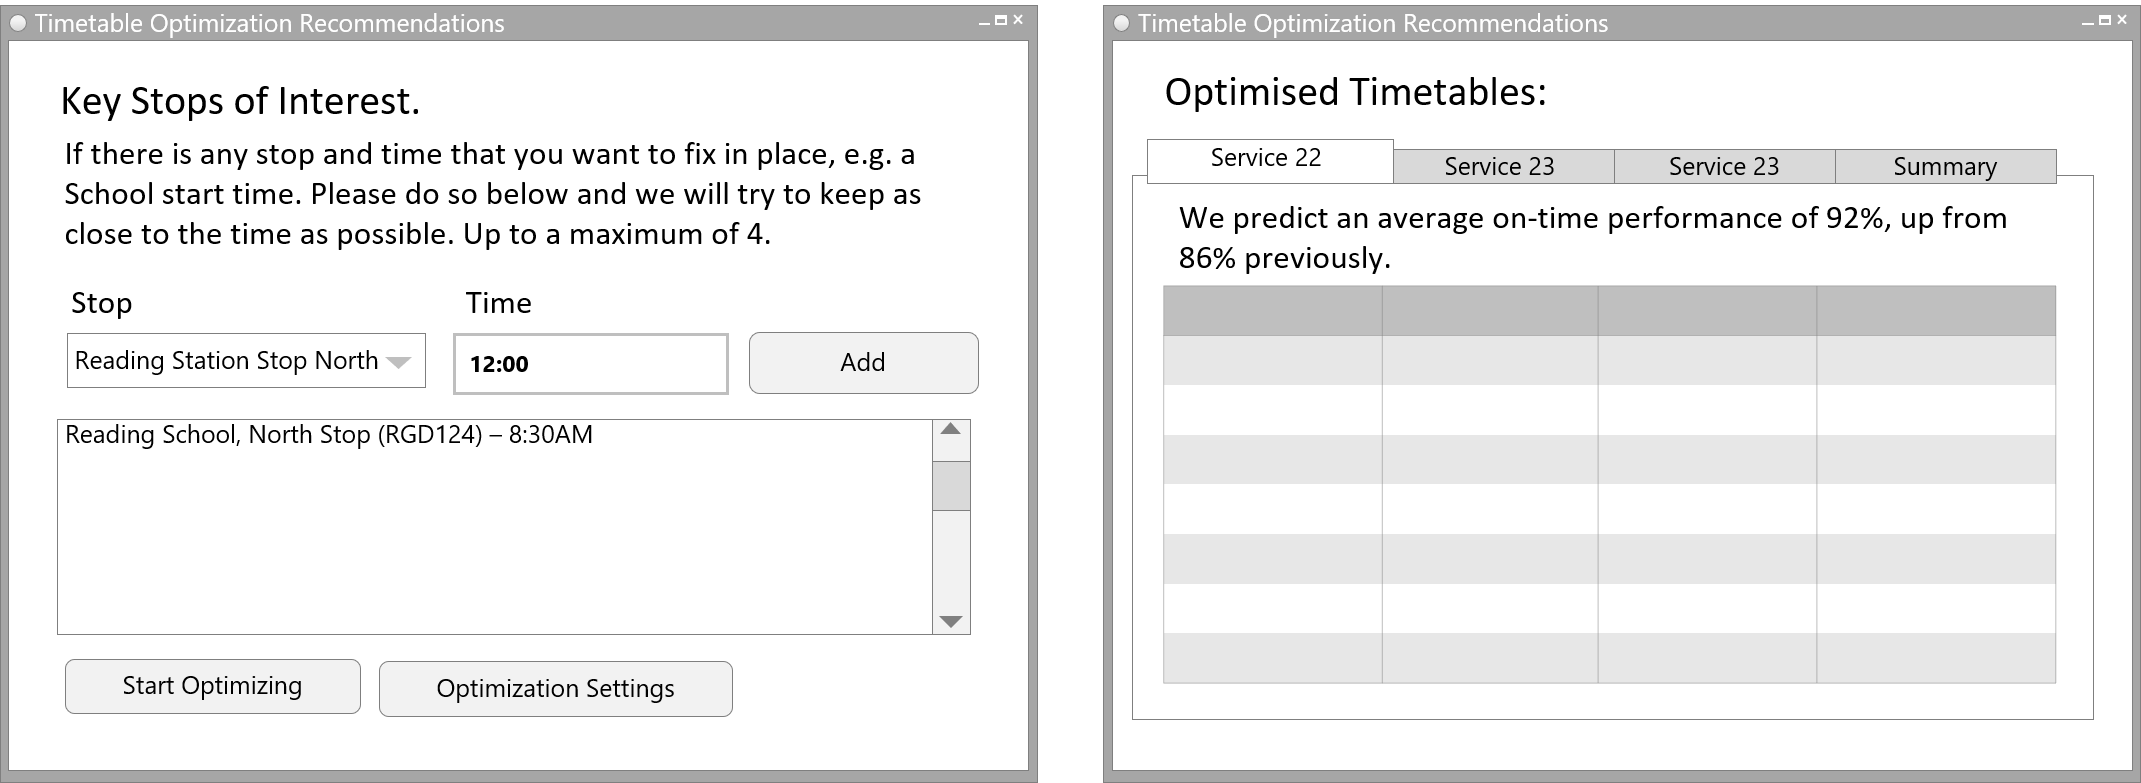
\includegraphics[height=110px]{images/GUI_2.png}
	\caption{GUI Design for Screens 4 to 5.}
	\label{fig:gui2}
\end{figure}

Finally, the user will be asked if there is any particular stop and timing pairs that they want to aim for and then the actual optimised timetable for each service will be outputted. Along with a set of estimated performance metrics. 


\subsection{Dataset}
For this project, I have decided to use the Reading Buses Open Data API (RBOD-API), due to its exemplary level of data access, providing a year's worth of historical bus timetable data, information on their bus stops and services operated and one month of historical GPS data, which can all be queried, by vehicle, service, stop and date. 

\par
Transport for London, West Midlands Transport, the National Bus Open Data Portal and Transport API UK, all provide a range of public transport APIs either for free or at a low-cost. Unfortunately, none of them provide historical data. While it is possible to request the data each day and make my own historical backlog of data, this would take several weeks to accumulate enough usable data and as such makes these impractical to use. All other bus operators in the UK are currently only providing a very limited set of public APIs, with the majority requiring authorization directly from the operator. Something I hope to avoid, as this could take several weeks to organise and get access. 


\par
Reading Buses does however not provide Automatic Passenger Counter (APC) information, while they do record ticket sales, this data is not publicly accessible, nor do they record when passengers are alighting. As I am not considering constraints of vehicle capacity and I am making the assumption that the waiting passenger flow-rate at a stop is roughly linearly consistent, I do not deem the lack of access to this data to be much of a hindrance. 


\subsubsection{Reading Buses Open Data API Library Design}
For the library, I planned on creating a .NET Standard 2.0 \CS, Class Library, this is because .NET standard provides the greatest level of portability between .NET versions and operating systems. The library should interface with all of the Reading Buses REST API, including: List of Bus Stops, Live Vehicle Positions, Live Journey Details, Stop Predictions, List of Services, Line Patterns, Timetabled Journeys, Tracking History and Vehicle Position History. While I do not envision needing all of these data-feeds they should be available to future proof. 


\par 
As the majority of the data provided by the API is in a proprietary format, as opposed to the standardised TransXChange format\cite{RN28}, I must create a custom solution to parse and interface with the API for my project. I propose a design, which has a main singleton controller, called ``operator'', which lets you get a list of bus services and stop locations, once you have a Bus Stop or Bus Service object you can then query further data about it. Which should be more intuitive than creating a class per API feed.

\subsection{Data-Schema Design}

\par
While this project utilises the RBOD-API, I wish for it to be portable to use with any operators API, particularly with the trend for bus open data APIs in recent years. While there are standardised ways for representing bus timetables and GPS data, I need for it to be formatted and processed in a useful way, so that it can be easily reasoned with. As such I have generated a data-scheme, by creating a set of interfaces, from which a class will implement to provide the functionality for an operators API.


\subsubsection{Bus Stop}

\begin{figure}[H]
	\centering
	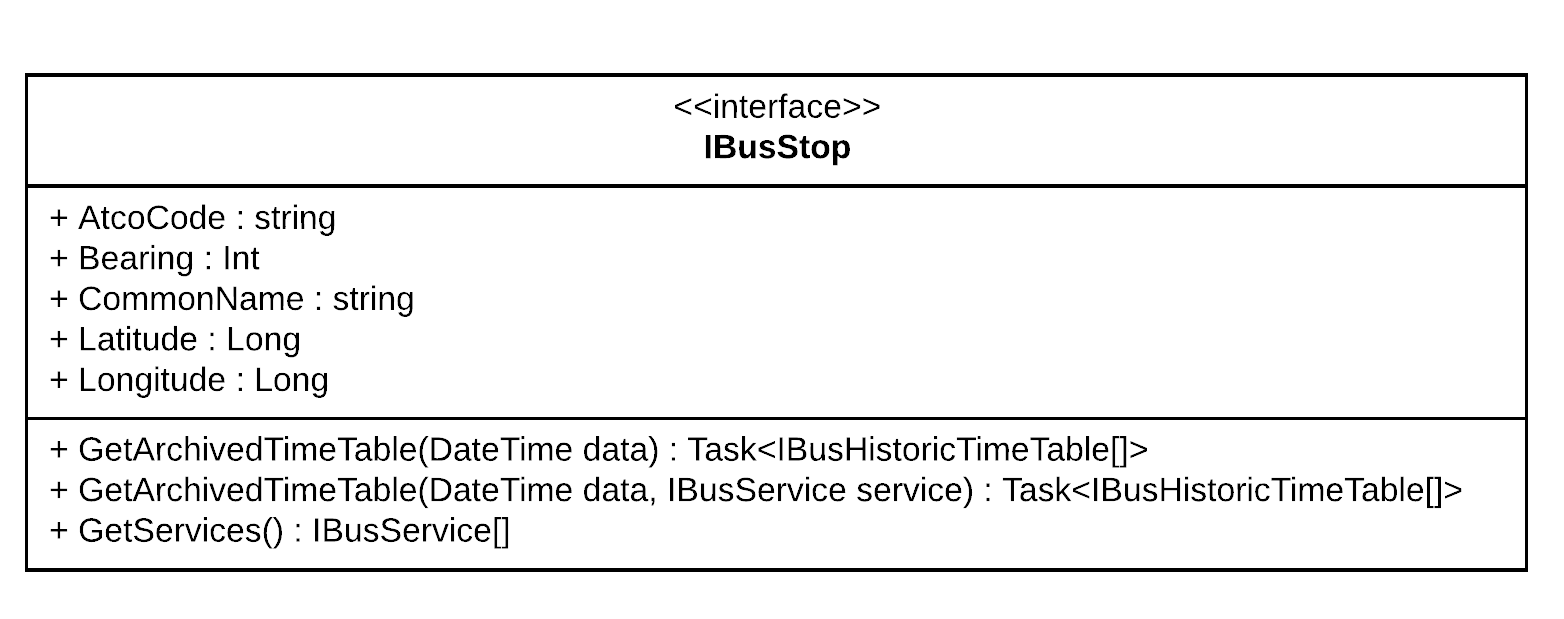
\includegraphics[width=300px]{images/CD_Stop.png}
	\caption{Bus Stop Data Class}
	\label{fig:busstopdata}
\end{figure}


Each bus stop, will have a NaPTAN ATCO Code, this is a unique alphanumeric string, that can identify any bus-stop in the UK. I will then store the stop's geographical location, from a longitude, latitude and bearing value. Finally, I will also store the services which visit the stop and provide the ability to get the archived timetable record data at the stop, with the ability to further filter it by service.  


\subsubsection{Bus Service}
\begin{figure}[H]
	\centering
	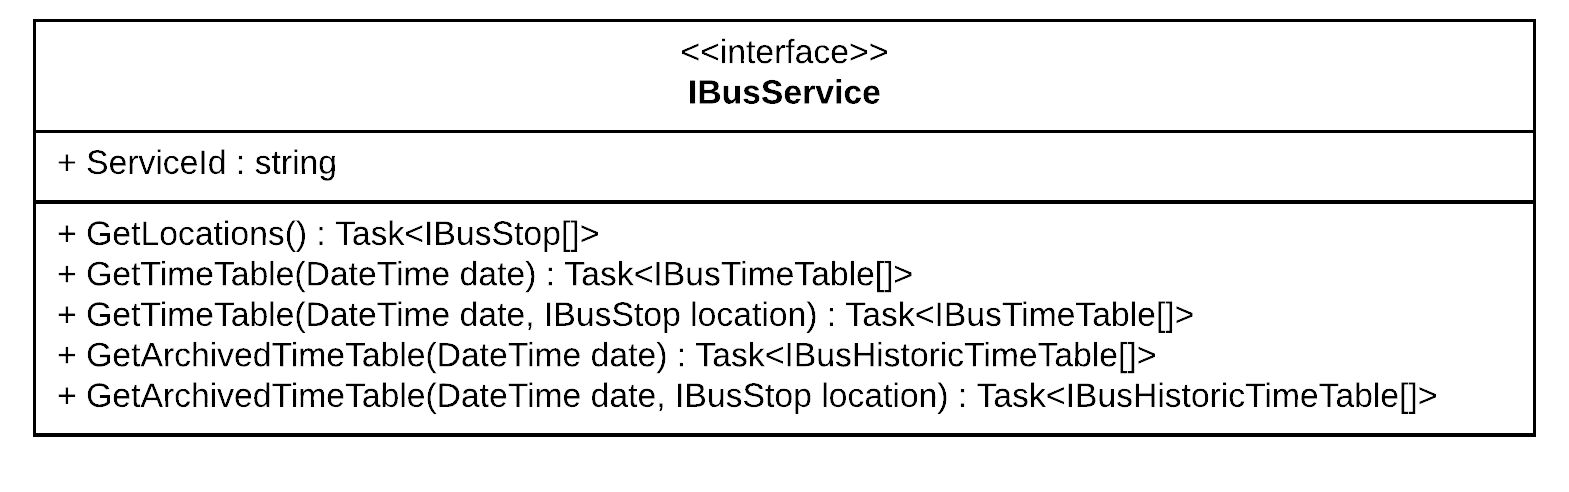
\includegraphics[width=300px]{images/CD_Service.png}
	\caption{Bus Service Data Class}
	\label{fig:busservicedata}
\end{figure}

Each bus service will have its own unique alphanumeric service ID, you will also be able to get a list of bus stops the service visits. Including the historical planned time table data and historical actual journey trip information, on a specific data and/or stop.


\subsubsection{Time Table Record}

\begin{figure}[H]
	\centering
	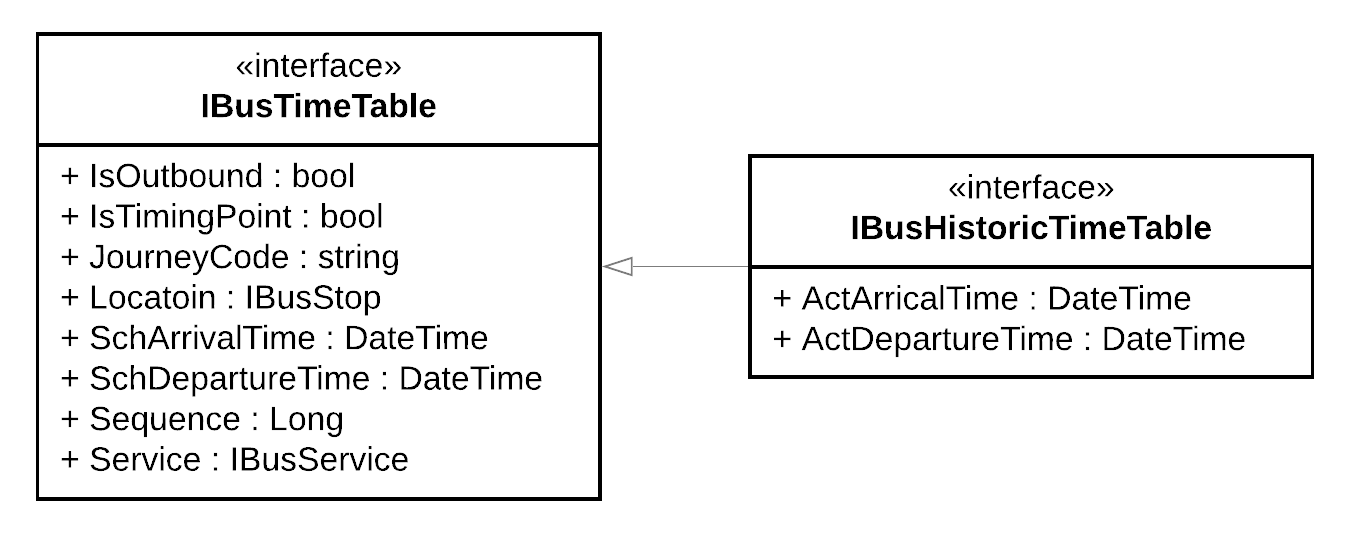
\includegraphics[width=300px]{images/CD_TimetableH.png}
	\caption{Bus Time Table and Historical Time Table Record Data Class}
	\label{fig:bustimetabledata}
\end{figure}

A timetable will be made up of an array of records, each record will include: if the service is travelling outbound, or inbound, the bus stop associated, is the stop a timing point, a journey code, which can be used to group together a set of records associated to one theoretical vehicle doing one loop of the route. The sequence code identifies the index of the bus stop along the route, for services which do not visit all the stops all the time, you may have a different sequence number per stop. Finally, you have an associated bus service object for each time-table record. A historical record, then inherits the base record and also includes the actual arrival and actual departure date and times. 

\subsection{Possible Simulation Methods}
To simulate how a bus service would have operated if the time table is changed, I should consider two main things, the estimated travel time between two stops at that specific time of day, as the traffic conditions change throughout the day and travel times will not be consistent. Secondly, I should consider the required dwell time at a stop at a specific time of day, to allow for passengers to alight or board at a stop in time; this will change throughout the day as passenger demand changes. As Reading Buses does not provide APC information, this will need to be estimated. 

\subsubsection{Travel Time Estimation}
\par 
To calculate the travel time between two stops, I will make the assumption that the historical travel times remain broadly consist throughout same parts of the year. I can also not only use the historical travel times of the specific service I am optimising for, but also look at the average travel times of any services which may go between the two stops. I will then look at the travel times of the vehicle before or after it, and depending upon how far the optimised bus has been moved forwards or backwards in the timetable I will proportionally grow or shrink the estimated travel time towards the nearest of the two travel averages. 

\par 
This method would not necessarily work where there is a lack of frequent data records, you are predicting the final or first record in the timetable or where you are making significant timetable changes. However, as one of my optimisation targets is to minimise large changes and I intend on using any service that goes between the two stops as data points, I hope there is enough data to be a reliable approximation. 

\subsubsection{Required Dwell Time Estimation}
\par
To calculate the historical dwell time, there are two situations to consider (1) A bus arrives at a stop earlier than scheduled, we must assume that it will wait at the stop until it was scheduled to leave (if at a timing point). So the time used will only be from the scheduled departure time, to the actual departure time. (2) If a bus turns up later than expected, then it should have left as soon as it could have left, in which case the actual arrival time and actual departure time can be used. Similarly, these times would be generated for any bus service that stops at the bus stop and a average weighting would be used for a new theoretical time.

\par 
The obvious downside of this is passengers can be alighting and boarding during the time in which a bus arrives early and was scheduled to have arrived. Furthermore, this assumes that all services are using similar vehicle designs (capacity, ticketing methods/machines and number of doors), so the time to board and alight can be compared. Additionally, you must assume that the flow rate of passengers arriving at the stop is roughly constant.

\par 

The total time for a bus to travel from one stop to another is therefore equal to \( Travel Time + Required Dwell Time\). This is just one possible proposed solution. I will need to prototype and test its feasibility before committing to it as my final design.





\subsection{Possible Optimisation Strategies}
Through my research on optimisation algorithms and related works I have identified the following promising types of algorithms I could use for this project. As such I have briefly explained them and their positives and negatives below:

\subsubsection{Genetic Algorithm}
By far the most popular optimisation technique currently researched in the bus timetable optimisation area is the use of various Genetic Algorithms (GA). GAs are based upon the theory of natural selection by Charles Darwin \cite{RN35}. You first start with multiple different solutions (known as chromosomes) to the problem and evaluate them to see how good they each are; only the evaluation function has any domain knowledge. The best chromosomes are then selected to ``breed'' with each other, which then produce a new solution mixing the different properties (genes) of both solutions. You then repeat the process again, until some condition such as time or number of populations has been reached and evaluate how good the produced solutions are. The hope is that by combining good solutions you produce even better solutions. Mutation can also occur, this is where a property of a chromosome is changed at random, doing this prevents for pre-mature convergence.

\par
GAs, can work faster and use less memory than other optimisation algorithms. However, randomisation means that it is not optimal and can get stuck on a local maxima, it can also be very difficult to be able to represent the problem as a bit string or otherwise. As such, due to their complexity, I have decided that this would be overly difficult for my skill set.  

\subsubsection{Integer Programming}
Another popular technique is Integer Programming (IP), this is when you formulate the problem as a mathematical representation, with an objective function to maximise and a set of linear constraints. This could further be advanced with Mixed-integer linear programming, where not all of the constraints must be integer. However, as IP is primarily used by people trying to represent the problem more as a mathematical model, I do not believe that this would be an appropriate solution. 

\subsubsection{Local Searches}
Another possibility is the use of a local search algorithms, these are heuristic methods, which apply local changes, without considering their effects at later stages, it simply tries to improve the current state and will do so until a time/attempt limit has elapsed, or a solution is deemed acceptable.

\paragraph{Hill-Climbing} is one form of local search optimisation, it starts with an arbitrary solution to the problem, for example the current timetable in place, and then tries to iteratively find a better solution through incremental changes \cite{RN36}. If the change produces a better solution then it is kept and another incremental change is made on-top of this solution, until no more improvements can be found. Hill-Climbing is a relatively simple, but popular search algorithm in AI. The problem with Hill-Climbing search is that if the problem is non-convex, which timetabling normally is, it can get stuck in a local optima inside of the search space where the best possible solution cannot be found. To get around this you can either use a new start location, increase the size of the neighbourhood to search, or use one the more advanced algorithms below.


\paragraph{Tabu-Search} (TS) is a form of meta-heuristic algorithm, proposed by Fred Glover in 1986, which tries to avoid entrapment in cycles by forbidding certain moves which have previously been visited \cite{RN35} \cite{RN37}. Tabu-search can accept non-improving solutions deterministically, so that it can escape from a local-optima and try to find better solutions further on. Tabu-search therefore needs to keep track in memory the states which have previously been visited to prevent re-visiting them. Tabu-search can be considered an extension of Hill-Climbing to allow it to escape from local-optimas


\par 
However, when you have a very large search space, or you are storing more attributes than are truly needed to represent the changes between stages. You can end up exhausting all your device's memory. It can also take a very long time just to check if you have visited the state before. Tabu-search can therefore, generate a generally good solution for optimisation problems. But Tabu list construction is problem specific and there is no guarantee of a global optimal solution. 


\paragraph{Simulated Annealing} (SA) is motivated by the physical annealing process, it mimics when a material is heated and slowly cooled down into a uniform structure \cite{RN35}. SA keeps track of a ``temperature'', when it is high the algorithm can accept a solution that is worst than our current one with a greater frequency. This allows it to escape from local optimus early in the execution. The temperature will gradually cool and as it does the probability of accepting a solution worse than the current reduces, which allows for it to gradually focus on a specific part of the search space.

\par 
SA is different to Hill-climbing because it will select its next move at random and decides whether to accept it with an acceptance function; whereas Hill-climbing will always choose the best move from all those available in the neighbourhood. This means that the results are generally not reproducible, as randomness is introduced. You should also keep track of what has been the best solution so far as the last solution is not necessarily going to be the best.


\subsection{Chosen Optimisation Strategy}
As per my work-plan I have decided to prototype with different optimisation strategies over the winter break. However, the current most promising solutions are Simulated Annealing and Tabu-Search. Both of these methods overcome the shortcomings of Hill-climbing but differs in their approaches, they are also popular and robust optimisation algorithms used in AI. Although, there is very limited documented usage of either being used for bus timetable optimisation, this however gives me a unique area of research to explore and evaluate later.


\section{Implementation}
The following section outlines, the work I have currently implemented and highlights the parts of particular technical complexity.


\subsection{Testing Strategy}
As planned, I have finished implementing the Reading Buses library, to test the library I have written Unit-Tests for each class, including any communication between them. Each test, has a ``live'' and ``dummy'' pair associated. The live tests, call upon the real API feed, making and receiving an actual request for data. This allows me to ensure the library is working as intended. Although, response times can be very long, taking up-to 15 minutes for all tests to complete. As such I also have associated dummy tests, these do not call upon the live server, instead they will call upon my hosted data-store of static results.

\par 
This has two main benefits, first the response times are significantly quicker, with the only bottle neck being the internet connection, as opposed to the server response time. Therefore, I can test and check the library is working much faster than beforehand, speeding up development. Secondly, if my dummy tests pass, but my live tests fail it allows for me to easily identify if the live server might have updated its data-schema, as opposed to an error being in my code. 

\par
A Continuous Integration Pipeline has also been set-up onto the master branch in GitHub, allowing me to quickly identify and fix any issues I may have accidentality introduced. A similar testing strategy will be deployed for the rest of the code-base, whilst also utilising user black-box testing for the graphical parts of the application.

\subsection{Data Caching}

\begin{figure}[H]
	\centering
	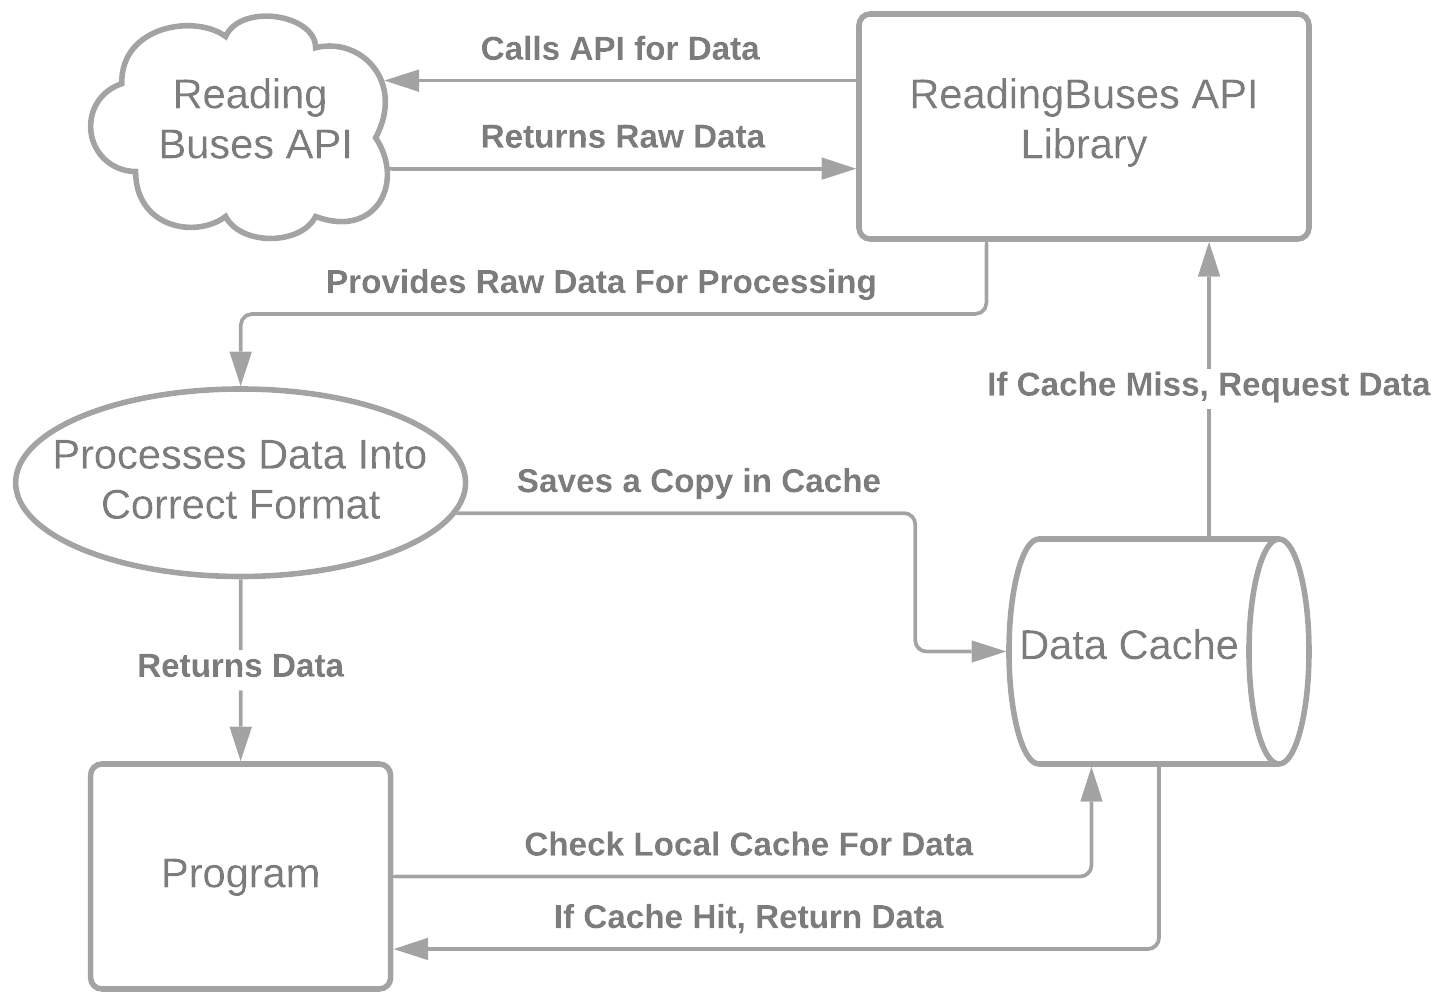
\includegraphics[width=200px]{images/data-diagram2.png}
	\caption{Data Caching System Architecture}
	\label{fig:cachingsystem}
\end{figure}


I identified that making data request to the API was a bottle-neck in the system, it would be impractical to request the volumes of data needed for the program every time it is run. Furthermore, historical data is not going to change after the date has taken place, because the same result is always going to be returned I can simply cache it locally. 



\par 
I therefore, implement a check before every call is made to an API server, is this request already cached locally, if so simply read from the file system, else make the API call and when the data is received, save a copy of it locally onto the device; as shown in Figure~\ref{fig:cachingsystem}.  The files are saved as ``.cache'' hidden files, in a directory path local to the executing program, called ``cache'', separated by the Operator Name, and Service ID path. By doing the caching checks inside of the library implementation, it abstracts it and allows for me to not have to worry about it elsewhere in the program. This also significantly speeds up the execution times for my program. 

\subsection{Asynchronous Data Management}
While I am caching the majority of the data, I cannot always assume a cache hit, and even if I have cached the file, reading from local storage and parsing the file into program memory can still take some time, especially for high-frequency services which will have a lot of data in a file to parse. As such I need to perform this work off of the main program thread, to prevent the GUI freezing later on and to allow for me the ability to carry out several requests to the API simultaneously.  


\par 
I have decided to achieve this with a Task-based Asynchronous Pattern (TAP)\cite{RN29}, through the use of \CS, System.Threading.Tasks.Task\textless TResult\textgreater  library. This allows for me to be able to easy compartmentalise work into tasks, which can then be queued, run asynchronously and managed to wait for some, or all, to complete with ease. This is particularly useful for when I want to get several dates' worth of data. Instead of doing each request sequentially and synchronously on the main thread, I can queue up all dates of tasks, and instruct them to all run concurrently on individual threads. With Tasks, abstracting much of the complexity away for me.  




\subsection{Identifying Timetable Patterns}
An important preliminary stage, was to work out at what points of the year the timetable has changed, so that I can produce an optimised timetable, for each grouping. Unfortunately, the Reading Buses API does not provide a simple way of achieving this. So instead, for each day I check does it match the timetable of another known timetable, if so add the date to the timetable, else it is a new timetable and so make a note of it. While this method is not overly efficient there is only ever going to be 365 days worth of data to check and as such $O(n^2)$ complexity should not be much of an issue. 


\subsection{Contingency Data-Backup}
In the unlikely event that the Reading Buses Open Data API becomes unavailable for whatever reason throughout the year, I have backed up a year's worth of historical timetable data for several popular routes throughout Reading. This has since been backed-up privately onto both cloud and local storage systems. This data can then simply be placed into the programs cache folder and I can continue relatively unaffected. 




\section{Progress}

I have officially, managed to complete everything I said I would have done from my initial work-plan. Completing my project proposal, producing my library to interface with the API, researching similar projects and investigating into weekly service patterns. 

\par 
However, the time it took to do some of the tasks was longer than anticipated, specifically the researching of similar projects, which was original assigned 4 weeks of work, but became closer to 5 weeks. Due primarily to the range and breadth of related projects and my indecisiveness in narrowing down my search sooner. 


\par 
With my greater understanding of the complexity and tasks at hand I have made some minor alterations to my original work plan, extending the time allocated to work on the main optimisation algorithm, as highlighted in Figure~\ref{fig:ganntchart} in red. I still hope to have the majority of the algorithm completed in the original time-slot. However, this extra time gives me the opportunity to evaluate it further, make any minor changes needed and could add in some extra slack time if needed.

\begin{figure}[H]
	\centering
	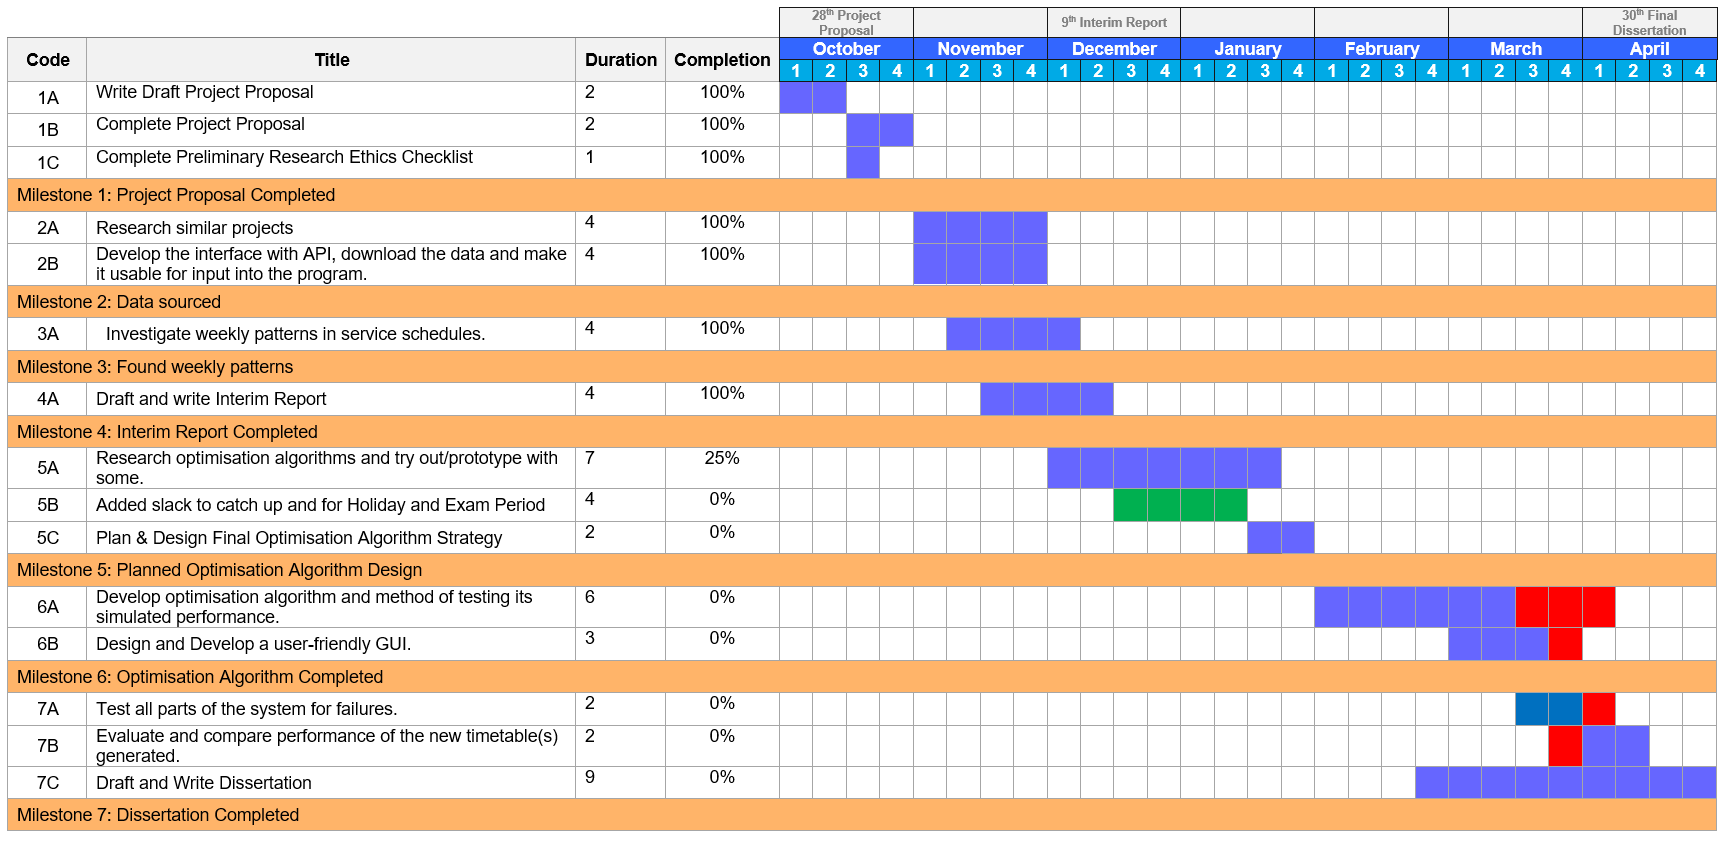
\includegraphics[width=400px]{images/ganntChartV3.png}
	\caption{Revised Gannt Work Plan}
	\label{fig:ganntchart}
\end{figure}



\subsection{Data Quality Issues} 
One area which could possibly hinder my progress going forwards, is the quality of the data. Initial inspections of the historical timetable data have highlighted some issues, for services which have a very high-frequency there is significant variation between the number of timetable records recorded day by day. When they should be generally consistent, as a services timetable should not change very often. This suggests that there may be some data missing, this could be because the drivers forgot to or incorrectly entered their vehicle journey code into the automatic vehicle location system (AVL), the vehicle was not equipped with an AVL device, connectivity issues or a service cancellation. 


\par 
A small number of records also appear to be erroneous, suggesting a bus had arrived significantly early or  late. This is particularly common for high-frequency services, where I suspect this is due to bus-bunching, where one bus catches up-to another and in some cases overtakes the service before it. In these situations an operator might opt to hold back a service, to enforce greater spacing between vehicles and enable the ability to return to more regular headway times. From a customer's prospective, they will have no knowledge of which vehicle should be in-front of which. Unfortunately, I do not believe the AVL back-end system is intelligent enough to detect two vehicles have effectively switched timetables mid service and I suspect this is the main source of error. Other possible reasons include driver error or connectivity issues. 

\subsubsection{Data Mitigation Strategy}
At the moment it is difficult to distinguish the extent of the missing data, due to its sheer volume. However, as this is only an undergraduate dissertation, not intended to be a commercially complete system, I shall not be performing any proactive data cleaning. Instead I intended to establish the effects caused by the missing data on the final solution and develop a mitigation strategy only if required. I hope, that while some days are missing data, there will be enough data from other weeks to still provide a complete representation.


\subsection{Project Management}
Throughout the project I have had bi-weekly meetings with my project supervisor, where I outlined the work I had completed in the previous two weeks and scope the work I intend to carry out for the following two weeks, using my work-plan to guide me. I started doing research and development concurrently where possible, first beginning development of the Reading Buses Open Data API Library; this was something I felt well-versed in doing. First I split up the problem into discrete parts and outlined to myself when I wished to have it completed by, in a SCRUM like agile approach.

\par 
For the remainder of the project I have decided to use Azure DevOps, as this can help me manage my work-items in a more efficient and structured way, particularly where I am less experienced in approach and the complexity of the task grows. Azure DevOps, allows for me to be able to effortlessly manage my work items and time, via the use of an easy to read and edit digital kanban like board. Where I can move work from different columns, such as To-do, In-Progress, Testing and Completed. I can also assign work-items properties such as, IDs, priorities, estimated time and dependencies/relations on other items. 

\par 
My Azure DevOps Project integrates well with Microsoft Excel and Project, which I have used to input in my current project timelines and work-items. After completing my prototyping during the winter break I shall further add to my list of work-items finalising it for the remainder of the project. I am choosing to use Azure DevOps as it is a popular choice in industry, I have previous development experience using it and it works well with my other technologies chosen (Visual Studio and Git.)

\par 
A continuous integration pipeline has also been set-up for my repository on GitHub, which enables me to double check my build is passing all of the required tests. 




\subsection{Contributions and Reflections}
Upon reflection, I am happy with the level of work and progress achieved, I have completed all of the tasks I set out for myself in the original work-plan and in doing so I have now built a solid ground-work and clear direction going forwards. Fully completing the Reading Buses Open Data API Library, implementation and testing. Coupled with my data caching design and implementation means I now have access to all of the required data for the project. Moreover, my data-mitigation strategy ensures that in the unlikely event the API is taken down I can still continue with my project relatively unaffected. 


\par 

An important lesson I learnt was with the researching of similar project ideas. There is already a lot of research carried out about the several areas of bus timetable optimisation. While researching allowed me to narrow down my proposed idea and approach, I think a more specific starting vision was required to help guide my direction of research. As I believe I spent too long focusing upon all the different areas, instead of targeting on a specific area sooner. The time needed to understand the complexity of the proposed methods was also greater than original anticipated. 


\par 
I have identified an area of study which has been under-researched and as such believe that my project does target a unique challenge. While there is a lot of work on urban bus-transit systems, from a route network design prospective, there is very limited research carried out on the relationship between multiple services timetables, in respect to a commonly used shared bus corridor. A particularly intriguing area of research, with Reading Borough Council, currently proposing further development into the town's bus lanes. I therefore believe I have a unique and interesting project for research and have a clear vision for how I wish to tackle the problem.

\vspace{2em}

% Do this to get it to show up in the contents page.
\phantomsection
\addcontentsline{toc}{section}{References}
\printbibliography %[heading=none]

\end{document}          
